
Cieľom tejto bakalárskej práce bolo spracovanie dát získaných z Nanopore sekvenovania
DNA za účelom modelovania narušenia informácie uchovávanej v DNA pamäti.

V rámci práce bol implementovaný celý pipeline spracovania dát — od stiahnutia
surových signálov zo sekvenovacieho zariadenia, cez basecalling pomocou nástroja
\textbf{Dorado}, až po zarovnanie a klastrovanie sekvencií pomocou algoritmu
\textbf{Clover}. Na základe zarovnaných reťazcov bol navrhnutý a implementovaný
vlastný multi-alignment algoritmus inšpirovaný beam search prístupom,
ktorý umožňuje určenie konsenzu pre skupiny DNA sekvencií.

Graf „Dĺžka reťazca vs počet DNA reťazcov“ prezentuje rozloženie dĺžok
zarovnaných DNA reťazcov a ich zastúpenie v spracovaných dátach.

\begin{figure}[h!]
    \centering
    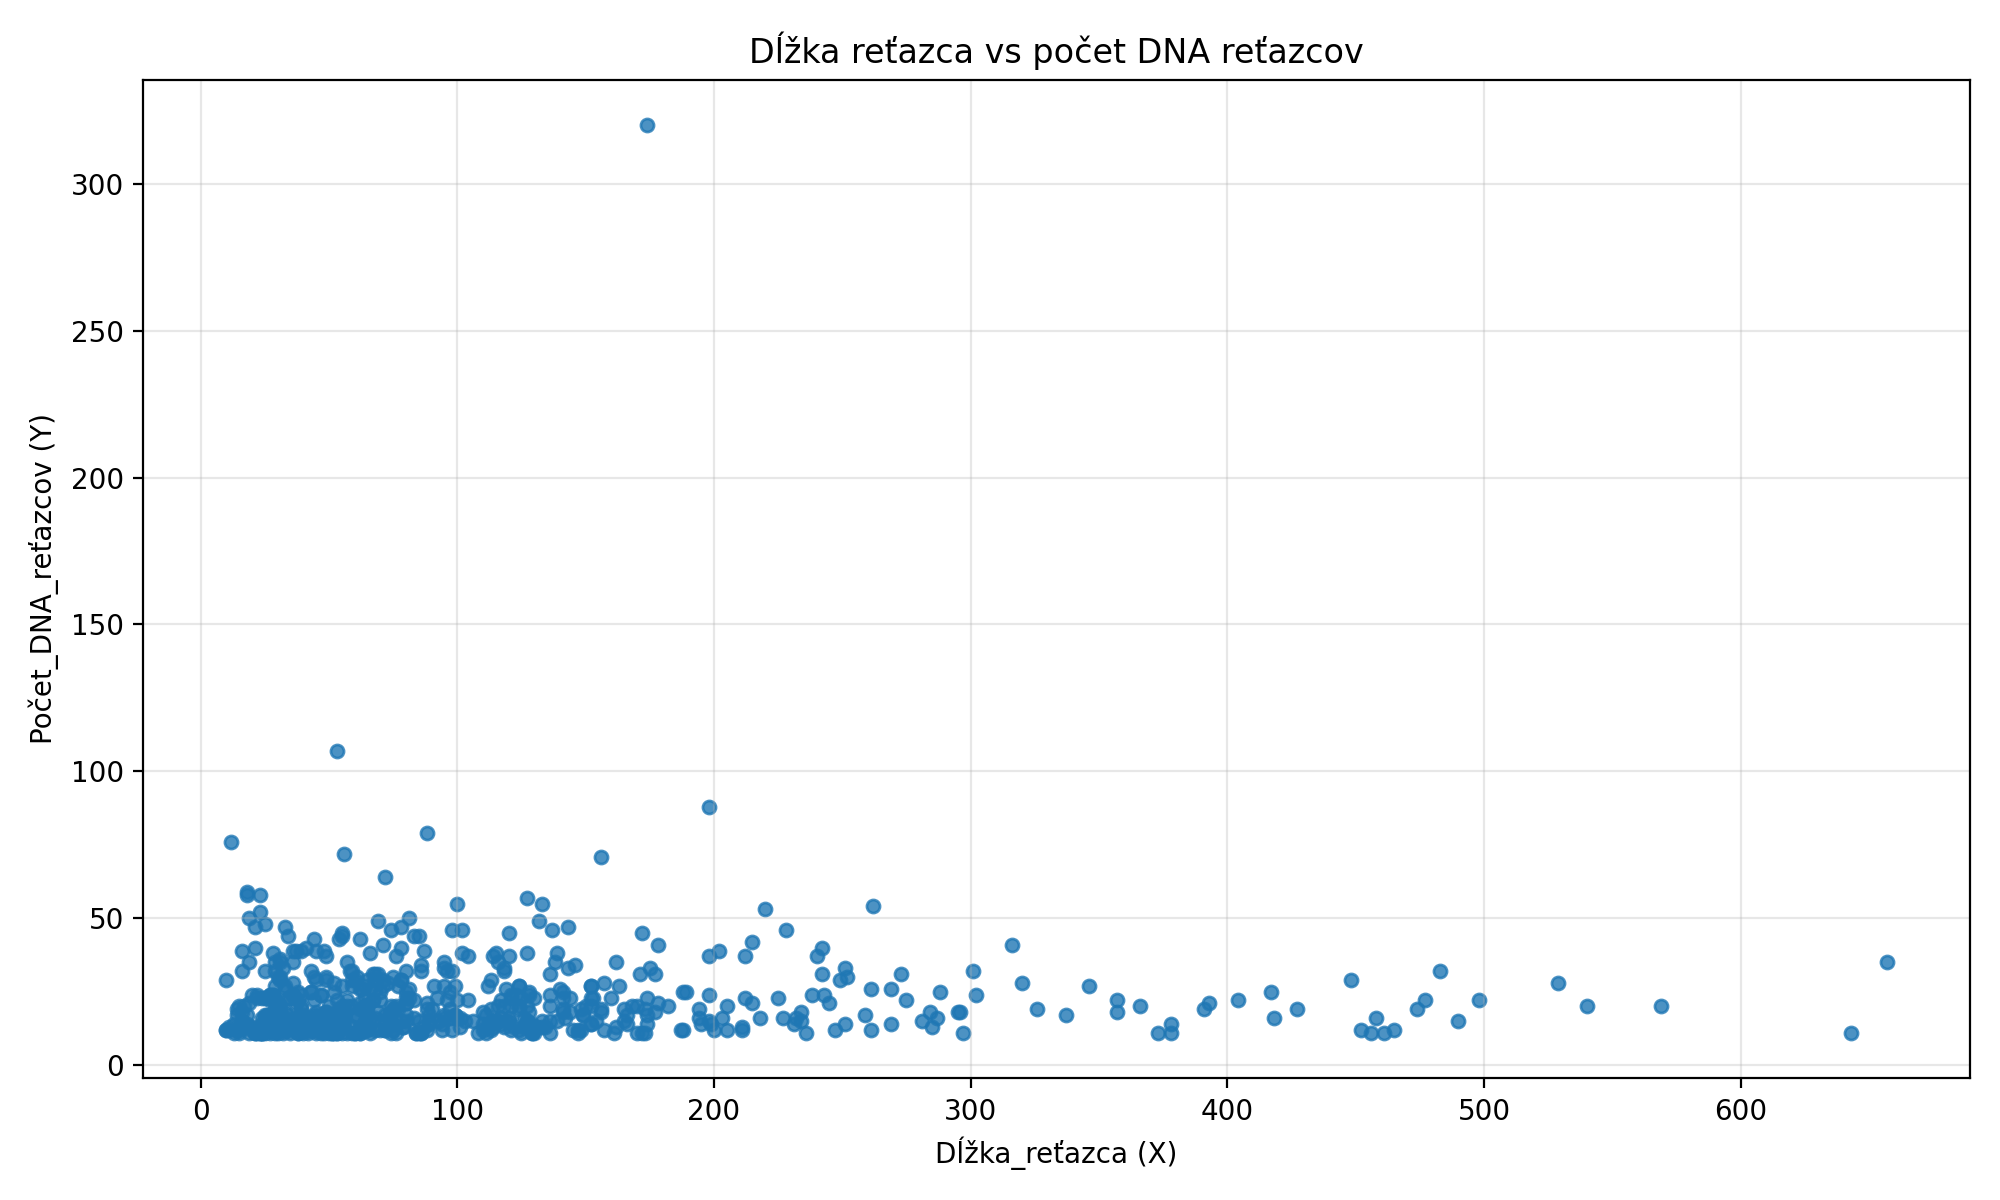
\includegraphics[width=\textwidth]{chapters/Figures/NajdeneZarovnanychRetazcov.png}
    \caption{Dĺžka reťazca vs počet DNA reťazcov}
    \label{fig:size_vs_num}
\end{figure}

Pri vyhodnotení výsledkov boli použité nasledovné kritériá:
\begin{itemize}
    \item dĺžka reťazca nad 100 bázových párov považovaná za dostatočnú,
    \item počet DNA reťazcov nad 10 ako prijateľný základ pre výpočet konsenzu,
    \item počet DNA reťazcov nad 50 ako veľmi silné zastúpenie zaručujúce spoľahlivý konsenzus.
\end{itemize}

Analýza ukázala, že v spracovaných dátach sa nachádzajú dostatočne dlhé reťazce
s dostatočným zastúpením, čo umožňuje spoľahlivý výpočet konsenzu a následné
modelovanie chybovosti Nanopore čítania. Získané výsledky tvoria základ
pre ďalší výskum v oblasti DNA pamätí, konkrétne pre charakterizáciu
chybových modelov pri Nanopore sekvenovaní.